% Vector UI notation shared by the question reference and worked UI answers.
% Coordinates are millimetres in each enclosing tikzpicture.
\newcommand{\uiEditField}[5]{%
  \draw (#1,#2) rectangle ++(#3,-#4);
  \node[anchor=west,inner sep=0pt] at ({#1+1.2},{#2-#4/2}) {#5};}
\newcommand{\uiReadField}[5]{%
  \draw (#1,#2) rectangle ++(#3,-#4);
  \begin{scope}
    \clip (#1,#2) rectangle ++(#3,-#4);
    \draw[black!65,line width=.3pt]
      ({#1+#3-4},{#2-#4}) -- ({#1+#3-1},{#2})
      ({#1+#3-1.5},{#2-#4}) -- ({#1+#3+1.5},{#2});
  \end{scope}
  \node[anchor=west,fill=white,inner xsep=.3pt,inner ysep=0pt]
    at ({#1+1.2},{#2-#4/2}) {#5};}
\newcommand{\uiReferenceExample}{%
  \begin{center}
  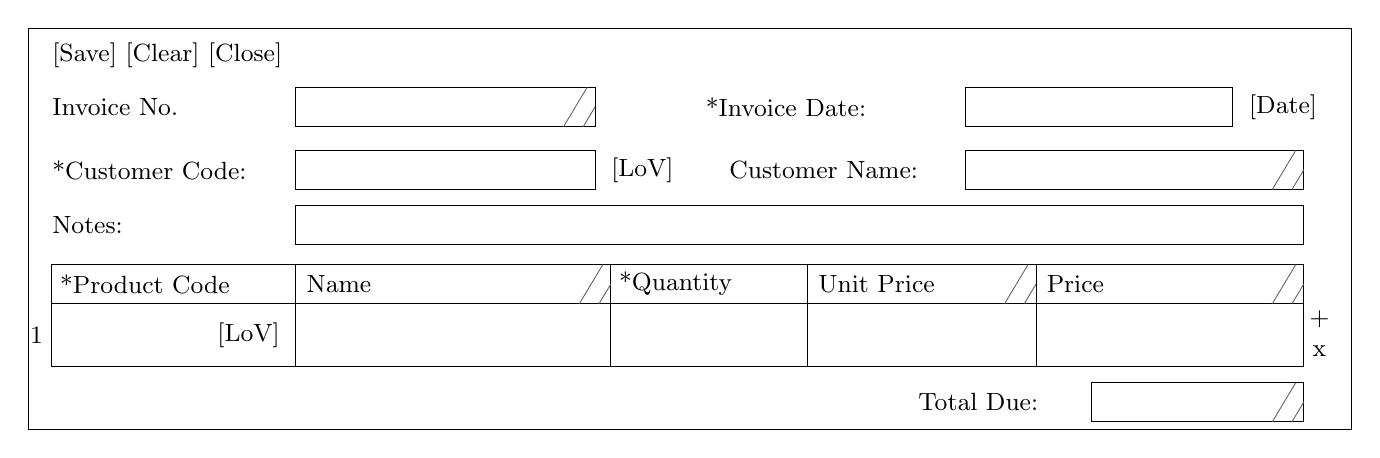
\begin{tikzpicture}[x=1mm,y=1mm,line width=.35pt,
    font=\fontsize{9}{11}\selectfont,every node/.append style={inner sep=0pt}]
  \draw (0,0) rectangle (168,-51);
  \node[anchor=west] at (3,-3.5) {[Save] [Clear] [Close]};
  \node[anchor=west] at (3,-10) {Invoice No.};
  \uiReadField{34}{-7.5}{38}{5}{}
  \node[anchor=west] at (86,-10) {*Invoice Date:};
  \uiEditField{119}{-7.5}{34}{5}{}
  \node[anchor=west] at (155,-10) {[Date]};
  \node[anchor=west] at (3,-18) {*Customer Code:};
  \uiEditField{34}{-15.5}{38}{5}{}
  \node[anchor=west] at (74,-18) {[LoV]};
  \node[anchor=west] at (89,-18) {Customer Name:};
  \uiReadField{119}{-15.5}{43}{5}{}
  \node[anchor=west] at (3,-25) {Notes:};
  \uiEditField{34}{-22.5}{128}{5}{}
  \draw (3,-30) rectangle (162,-43);
  \foreach \x in {34,74,99,128}{\draw (\x,-30)--(\x,-43);}
  \draw (3,-35)--(162,-35);
  \node[anchor=west] at (4,-32.5) {*Product Code};
  \uiReadField{34}{-30}{40}{5}{Name}
  \node[anchor=west] at (75,-32.5) {*Quantity};
  \uiReadField{99}{-30}{29}{5}{Unit Price}
  \uiReadField{128}{-30}{34}{5}{Price}
  \node[anchor=west] at (.2,-39) {1};
  \node[anchor=east] at (32,-39) {[LoV]};
  \node at (164,-37) {+};\node at (164,-41) {x};
  \node[anchor=west] at (113,-47.5) {Total Due:};
  \uiReadField{135}{-45}{27}{5}{}
  \end{tikzpicture}
  \end{center}}
